\documentclass[11pt,a4paper]{article}
\usepackage[utf8]{vietnam}
\usepackage{fontenc}
\usepackage{amsmath}
\usepackage{amsfonts}
\usepackage{amssymb}
\usepackage{graphics}
\usepackage{cases} 
\usepackage{enumitem}
\usepackage{fancyhdr}
\usepackage{xcolor}
\usepackage{mdframed}
\usepackage{colortbl}
\usepackage{fontawesome}
\usepackage{tikz}
\usepackage{setspace}
\usepackage{listings}
\definecolor{dgray}{gray}{0.35} % colour of R comments
\definecolor{lgray}{gray}{0.9999} % background colour of R-code
\usetikzlibrary{patterns}
\usetikzlibrary{calc,angles}
\usepackage[left= 2cm, right = 2cm, top = 2cm, bottom = 2cm]{geometry}
\usepackage{scalefnt}
\usepackage{fancybox}
\usepackage{multirow}
\usepackage{pgfplots}
\usepackage{hyperref}
\definecolor{dkgreen}{rgb}{0,0.6,0}
\definecolor{gray}{rgb}{0.5,0.5,0.5}
\definecolor{mauve}{rgb}{0.58,0,0.82}
\pagestyle{fancy}
\fancyhf{}
%\rhead{\textit{Nhóm 18}}
\lhead{\textit{Bài Tập Lớn Đại Số Tuyến Tính}}
\lfoot{\textit{Nhóm 5-L13}}
\rfoot{Trang \thepage}
\renewcommand{\footrulewidth}{0.4pt}
\renewcommand{\headrulewidth}{0.4pt}
\lstset{ % setting appearance of R-code
	language=C, % setting language R
	basicstyle=\ttfamily\small, % font and size of R-code
	backgroundcolor=\color{lgray}, % background colour of R-code
	commentstyle=\ttfamily\small\itshape\color{dgray}, % colour of R comments
	showstringspaces=false, % forbidding the highlighting of spaces
	% numbering on the left
	% cumulative numbering of rows in consecutive uses of lstlisting environment
	breaklines=T} % automatic line breaks of code at the end of a line
\newmdenv[linewidth=0.6pt,linecolor=black,skipabove=\topsep,skipbelow=\topsep,
leftmargin=-5pt,rightmargin=-5pt,
innerleftmargin=5pt,innerrightmargin=5pt]{mybox}
\setlist{nolistsep}
\newcommand\tab[1][0.7cm]{\hspace*{#1}}
\setlength{\parindent}{0pt}
\begin{document}
	\begin{titlepage}
		\begin{center}
			ĐẠI HỌC QUỐC GIA THÀNH PHỐ HỒ CHÍ MINH\\
			TRƯỜNG ĐẠI HỌC BÁCH KHOA\\
			KHOA KHOA HỌC ỨNG DỤNG\\
		\end{center}
		\begin{figure}[h!]
			\begin{center}
				\vspace{0.5cm}
				
\includegraphics[width=3cm]{hcmut.png}
			\end{center}
		\end{figure}
		\vspace{2cm}
		\begin{center}
			\begin{tabular}{c}
				\textbf{{\Large BÀI TẬP LỚN ĐẠI SỐ TUYẾN TÍNH}}\\ \\
				\hline
				\\ \\
				\textbf{\huge{\textcolor{blue}{PHÂN TÍCH SVD }}} \\
				\textbf{\huge{\textcolor{blue}{KHỬ NHIỄU ÂM THANH}}} \\
				\\ \\
				\hline
				\textbf{{\Large Nhóm 5-L13}}
				%	\textbf{{\Large NHÓM 18}}\\ \\
			\end{tabular}
		\end{center}
		\vspace{3cm}
		
		\begin{table}[h]
			\begin{tabular}{rrl}
				\hspace{5 cm} & \textbf{Giảng viên hướng dẫn}: &Nguyễn Hữu Hiệp\\
				
				%& \textbf{Sinh viên thực hiện}: & Huỳnh Nga  -- 2111818 \\
				
				%& & Trương YY Nhi  -- 2111947  \\
				%& & Nguyễn Thành Phát  -- 2111982 \\
				%& & Lê Quốc Tài  -- 2112223 \\
				%& & Nguyễn Minh Mỹ Tâm  -- 2112238 \\
				%& & Nguyễn Hồ Ngọc Thiện  -- 2112354 \\
				%& & Nguyễn Minh Thư  -- 2112405 \\
			\end{tabular}
		\end{table}
	\begin{center}
		\begin{tabular}{|c|l|c|c|}
			\hline
			\textbf{STT}  &\textbf{ Họ và tên} & \textbf{MSSV} & \textbf{Hoàn thành}\\
			\hline
			1 & Huỳnh Nga  & 2111818 & 100\% \\
			\hline
			2 & Trương YY Nhi & 2111947 & 100\% \\
			\hline
			3 & Nguyễn Thành Phát & 2111982 & 100\% \\
			\hline
			4 & Lê Quốc Tài & 2112223 & 100\%\\
			\hline 
			5 & Nguyễn Minh Mỹ Tâm & 2112238  & 100\%\\
			\hline
			6 & Nguyễn Hồ Ngọc Thiện & 2112354 & 100\%\\
			\hline
			7 & Nguyễn Minh Thư & 2112405 & 100\%\\
			\hline
		\end{tabular}
	\end{center}
		\vspace{1cm}
		\begin{center}
			{\footnotesize Ho Chi Minh City, 2022}
		\end{center}
	\end{titlepage}
	\newpage
	
	\tableofcontents
	
	\newpage
	\section{CƠ SỞ LÍ THUYẾT CỦA PHÂN TÍCH SVD}
\subsection{Giới thiệu}
Trong Đại số tuyến tính ta thường gặp các dạng bài toán chéo hóa ma trận: Với một ma trận $A\in \mathbb{R}^{n\times n}$ được gọi là \textit{chéo hóa} được (diagonalizable) nếu tồn tại ma trận đường chéo \textbf{D} và ma trận khả nghịch \textbf{P} sao cho:\\

\begin{center}
	$A=PDP^{-1}$ (1)
\end{center}



Số lượng phần tử khác 0 của ma trận đường chéo \textbf{D}
chính là rank của ma trận \textbf{A}.\\
Nhân cả hai vế của (1) với \textbf{P} ta có:\\

\begin{center}
	$AP=PD$ (2)
\end{center}
Gọi $p_i$, $d_i$ lần lượt là cột thứ i của ma trận $\textbf{P}$ và \textbf{D}. Vì mỗi một cột của vế trái và vế phải của (2) phải bằng nhau, ta sẽ có:\\
\begin{center}
	$A_{p_i}=Pd_i=d_{ii}p_i$ (3)
\end{center}
với $d_{ii}$ là phần tử thứ i của $p_i$\\
\\ 
Dấu bằng thứ hai xảy ra vì \textbf{D} là ma trận đường chéo, tức $d_i$ chỉ có thành phần $d_{ii}$ là khác 0. Biểu (3) chỉ ra rằng mỗi phần tử $d_{ii}$ phải trị riêng (eigenvalue) của \textbf{A} và mỗi vector cột $p_i$, phải là một vector riêng (eigenvector) của \textbf{A} ứng với trị riêng $d_{ii}$\\
\\
Cách phân tích một ma trận vuông thành nhân tử như (1) còn được gọi là Eigen Decomposition. \\
\\
Một điểm quan trọng là cách phân tích như (1) chỉ được áp dụng với ma trận vuông và không phải lúc nào cũng tồn tại. Nó chỉ tồn tại nếu ma trận \textbf{A} có n vector riêng độc lập tuyến tính, vì nếu không thì không tồn tại ma trận \textbf{P} khả nghịch. Thêm nữa, cách phân tích này cũng không phải là duy nhất vì nếu \textbf{P, D} thỏa mãn (1) thì \textbf{kP, D} cũng thỏa mãn với k là một số thực khác 0 bất kỳ\\
\\
Việc phân tích một ma trận ra thành tích của nhiều ma trận đặc biệt khác (Matrix Factorization hoặc Matrix Decomposition) mang lại nhiều ích lợi quan trọng mà các bạn sẽ thấy: giảm số chiều dữ liệu, nén dữ liệu, tìm hiểu các đặc tính của dữ liệu, giải các hệ phương trình tuyến tính, clustering, và nhiều ứng dụng khác. Recommendation System cũng là một trong rất nhiều ứng dụng của Matrix Factorization.\\
\\
Một trong những phương pháp Matrix Factorization rất đẹp của Đại số tuyến tính. Phương pháp đó có tên là Singular Value Decomposition (SVD). Mọi ma trận, không nhất thiết là vuông, đều có thể được phân tích thành tích của ba ma trận đặc biệt.
\newpage 
\subsection{Kiến thức liên quan đại số tuyến tính} 
\subsubsection{Trị riêng và vector riêng} 
Cho một ma trận vuông $A\in \mathbb{R}^{n\times n}$, nếu số vô hướng $\lambda$ và vector $x \neq 0 \in \mathbb{R}^n$ thỏa mãn:\\
\begin{center}
	$Ax=\lambda x$    
\end{center}
thì $\lambda$ được gọi là một trị riêng của \textbf{A} và x được gọi là vector riêng tương ứng với trị riêng đó. \\
Một vài tính chất: \\
1. Nếu x là một vector riêng của \textbf{A} ứng với $\lambda$ thì $kx, k\neq 0$ cũng là vector riêng ứng với trị riêng đó.\\
2. Mọi ma trận vuông bậc n đều có n trị riêng (kể cả lặp) và có thể là các số phức\\
3. Với ma trận đối xứng, tất cả các trị riêng đều là các số thực.\\
4. Với ma trận xác định dương, tất cả các trị riêng của nó đều là các số thực dương. Với ma trận nửa xác định dương, tất cả các trị riêng của nó đều là các số thực không âm.\\
Tính chất cuối cùng có thể được suy ra từ định nghĩa của ma trận (nửa) xác định dương. Thật vậy, gọi $u \neq 0$ là vector riêng ứng với một trị riêng $\lambda$ của ma trận \textbf{A} xác định dương, ta có:
\begin{center}
	$Au=\lambda u \Rightarrow u^{T}Au=\lambda u^{T}u=\lambda ||u||_2^2$
\end{center}
Vì \textbf{A} là nửa xác định dương nên với mọi $u \neq 0: u^{T}Au \geq 0$; $u \neq 0$ nên $||u||_2^2 > 0$. Từ đó suy ra $\lambda $ là một số không âm\\

\subsubsection{Hệ trực giao và trực chuẩn}
%\begin{figure}[!ht]
%	\centering
%	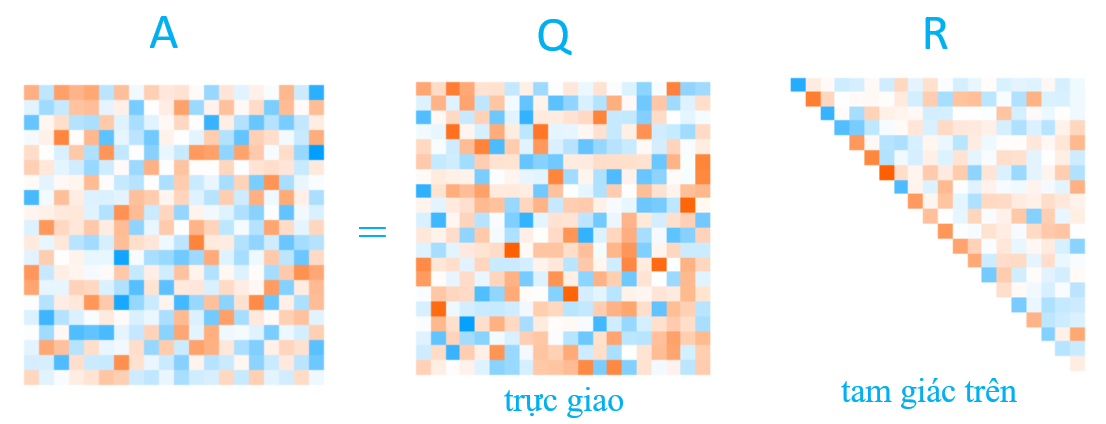
\includegraphics[scale=0.4]{ytuong}
%\caption{\textit{Conversion between human, high-level, assembly, and machine language}}\label{fig:Picture}
%\end{figure}
Một hệ cơ sở $u_1, u_2, ...,u_m \in \mathbb{R}^m$ được gọi là trực giao (orthogonal) nếu mỗi vector là khác 0 và tích của hai vector khác nhau bất kỳ bằng 0:\\
\begin{center}
	$u_i \neq 0; u_i^{T}u_j=0  \forall  1\leq i \neq j\leq m	$
\end{center}
Một hệ cơ sở $u_1, u_2, ...,u_m \in \mathbb{R}^m$ được gọi là trực chuẩn (orthonormal) nếu nó là một hệ trực giao và độ dài Euclidean (norm 2) của mỗi vector bằng 1:\\

% cách dùng
\begin{center}
	$u_i^{T}u_j=$
	\begin{cases}
		1\hspace{0.2cm} if \hspace{0.2cm} i=j\\
		0 \hspace{0.2cm} otherwise
	\end{cases}
\end{center}
Gọi $U=[u_1, u_2,...,u_m] $ với $u_1, u_2,...,u_m \in \mathbb{R}^m$ là trực chuẩn, từ (4) có thể suy ra:\\
\begin{center}
	$UU^{T}=U^{T}U=I$
\end{center}
trong đó $I$ là ma trận đơn vị bậc m. Ta gọi U là ma trận trực giao (orthogonal matrix). Ma trận loại này không dược gọi là ma trận trực chuẩn, không có định nghĩa cho ma trận trực chuẩn\\
Một vài tính chất: \\
1. $\mathbf{U}^{-1} = \mathbf{U}^T$: nghịch đảo của một ma trận trực giao chính là chuyển vị của nó\\
2. Nếu \mathbf{U} là ma trận trực giao thì chuyển vị của nó $\mathbf{U}^T$ cũng là một ma trận trực giao.\\
3. Định thức (determinant) của ma trận trực giao bằng $1$ hoặc $-1$. Điều này có thể suy ra từ việc $\det(\mathbf{U}) = \det(\mathbf{U}^T)$ và $\det(\mathbf{U}) \det(\mathbf{U}^T) = \det(\mathbf{I}) = 1$\\
4. Ma trận trực giao thể hiện cho phép xoay (rotate) một vector. Giả sử có hai vector $\mathbf{x,y} \in \mathbb{R}^m$ và ma trận trực giao $\mathbf{U} \in \mathbb{R}^{m \times m}$. Dùng ma trận này để xoay hai vector trên ta được $Ux, Uy$. Tích vô hướng của hai vector mới là:\\
\begin{center}
	$
	(\mathbf{Ux})^T (\mathbf{Uy}) = \mathbf{x}^T \mathbf{U}^T \mathbf{Uy} = \mathbf{x}^T\mathbf{y}$\\
\end{center}
như vậy phép xoay không làm thay đổi tích vô hướng giữa hai vector.\\
5. Giả sử $\hat{\mathbf{U}} \in \mathbb{R}^{m \times r}, r < m$  là môt ma trận con của ma trận trực giao $\mathbf{U}$  được tạo bởi r cột của $\mathbf{U}$, ta sẽ có $\hat{\mathbf{U}}^T\hat{\mathbf{U}} = \mathbf{I}_{r}$. Việc này có thể suy ra từ (4)

\subsection{Singular Value Decomposition}
Phương pháp \textit{phân tích suy biến} (singular value decomposition) được viết tắt là SVD là một trong những phương pháp thuộc nhóm \textit{matrix factorization} được phát triển lần đầu bởi những nhà hình học vi phân. Ban đầu mục đích của phương pháp này là tìm ra một phép xoay không gian sao cho tích vô hướng của các vector không thay đổi. Từ mối liên hệ này khái niệm về ma trận trực giao đã hình thành để tạo ra các phép xoay đặc biệt. Phương pháp SVD đã được phát triển dựa trên những tính chất của ma trận trực giao và ma trận đường chéo để tìm ra một ma trận xấp xỉ với ma trận gốc. Phương pháp này sau đó đã được ứng dụng rộng rãi trong các lĩnh vực như hình học vi phân, hồi qui tuyến tính, xử lý hình ảnh, khử nhiễu âm thanh, clustering, các thuật toán nén và giảm chiều dữ liệu, và đặc biệt đặc biệt hiệu quả trong các bài toán recommendation.\\
\\
Một số thông tin chung nhất về thuật toán SVD: Phương pháp SVD sẽ tìm ra một lớp các ma trận xấp xỉ tốt nhất với một ma trận cho trước dựa trên khoảng cách norm Frobenios giữa 2 ma trận. Người ta đã chứng minh được rằng ma trận xấp xỉ tốt nhất được biểu diễn dưới dạng tích của 3 ma trận rất đặc biệt bao gồm 2 ma trận trực giao (orthogonal matrix) và 1 ma trận đường chéo (diagonal matrix). Quá trình nhân ma trận thực chất là quá trình biến đổi các điểm dữ liệu của ma trận gốc thông qua những phép xoay trục (rotation) và phép thay đổi độ lớn (scaling) và từ đó tạo ra những điểm dữ liệu mới trong không gian mới. Điều đặc biệt của ma trận đường chéo đó là các phần tử của nó chính là những giá trị riêng của ma trận gốc. Những điểm dữ liệu trong không gian mới có thể giữ được 100\% thông tin ban đầu hoặc chỉ giữ một phần lớn thông tin của dữ liệu ban đầu thông qua các phép truncate SVD. Bằng cách sắp xếp các trị riêng theo thứ tự giảm dần trên đường chéo chính thuật toán SVD có thể thu được ma trận xấp xỉ tốt nhất mà vẫn đảm bảo giảm được hạng của ma trận sau biến đổi và kích thước các ma trận nhân tử nằm trong giới hạn cho phép. Do đó nó tiết kiệm được thời gian và chi phí tính toán và đồng thời cũng tìm ra được một giá trị dự báo cho ma trận gốc với mức độ chính xác cao.
\subsubsection{Phát biểu SVD}
Một ma trận $\mathbf{A}_{m \times n}$  bất kỳ đều có thể phân tích thành dạng:\\
\begin{center}
	$
	\mathbf{A}_{m \times n} = \mathbf{U}_{m \times m}\mathbf{\Sigma}_{m \times n} (\mathbf{V}_{n \times n})^T ~~~~ (5)$
\end{center}
Trong đó, $\mathbf{U}, \mathbf{V}$  là các \textit{ma trận trực giao}, $\mathbf{\Sigma}$ là ma trận đường chéo không vuông với các phần tử trên đường chéo $\sigma_1 \geq \sigma_2 \geq \dots \geq\sigma_r \geq 0 = 0 = \dots = 0$  và r là rank của ma trận $\mathbf{A}$. Lưu ý rằng mặc dù $\Sigma$  không phải ma trận vuông, ta vẫn có thể coi nó là ma trận chéo nếu các thành phần khác không của nó chỉ nằm ở vị trí \textit{đường chéo}, tức tại các vị trí có chỉ số hàng và chỉ số cột là như nhau.\\
Số lượng các phần tử khác 0 trong $\Sigma$ chính là rank của ma trận $\mathbf{A}$.\\

\\
\textbf{\textcolor{blue}{Mô tả SVD của ma trận A trong trường hợp m<n (m=4 và n=8)}} \\
\begin{figure}[!ht]
	\centering
	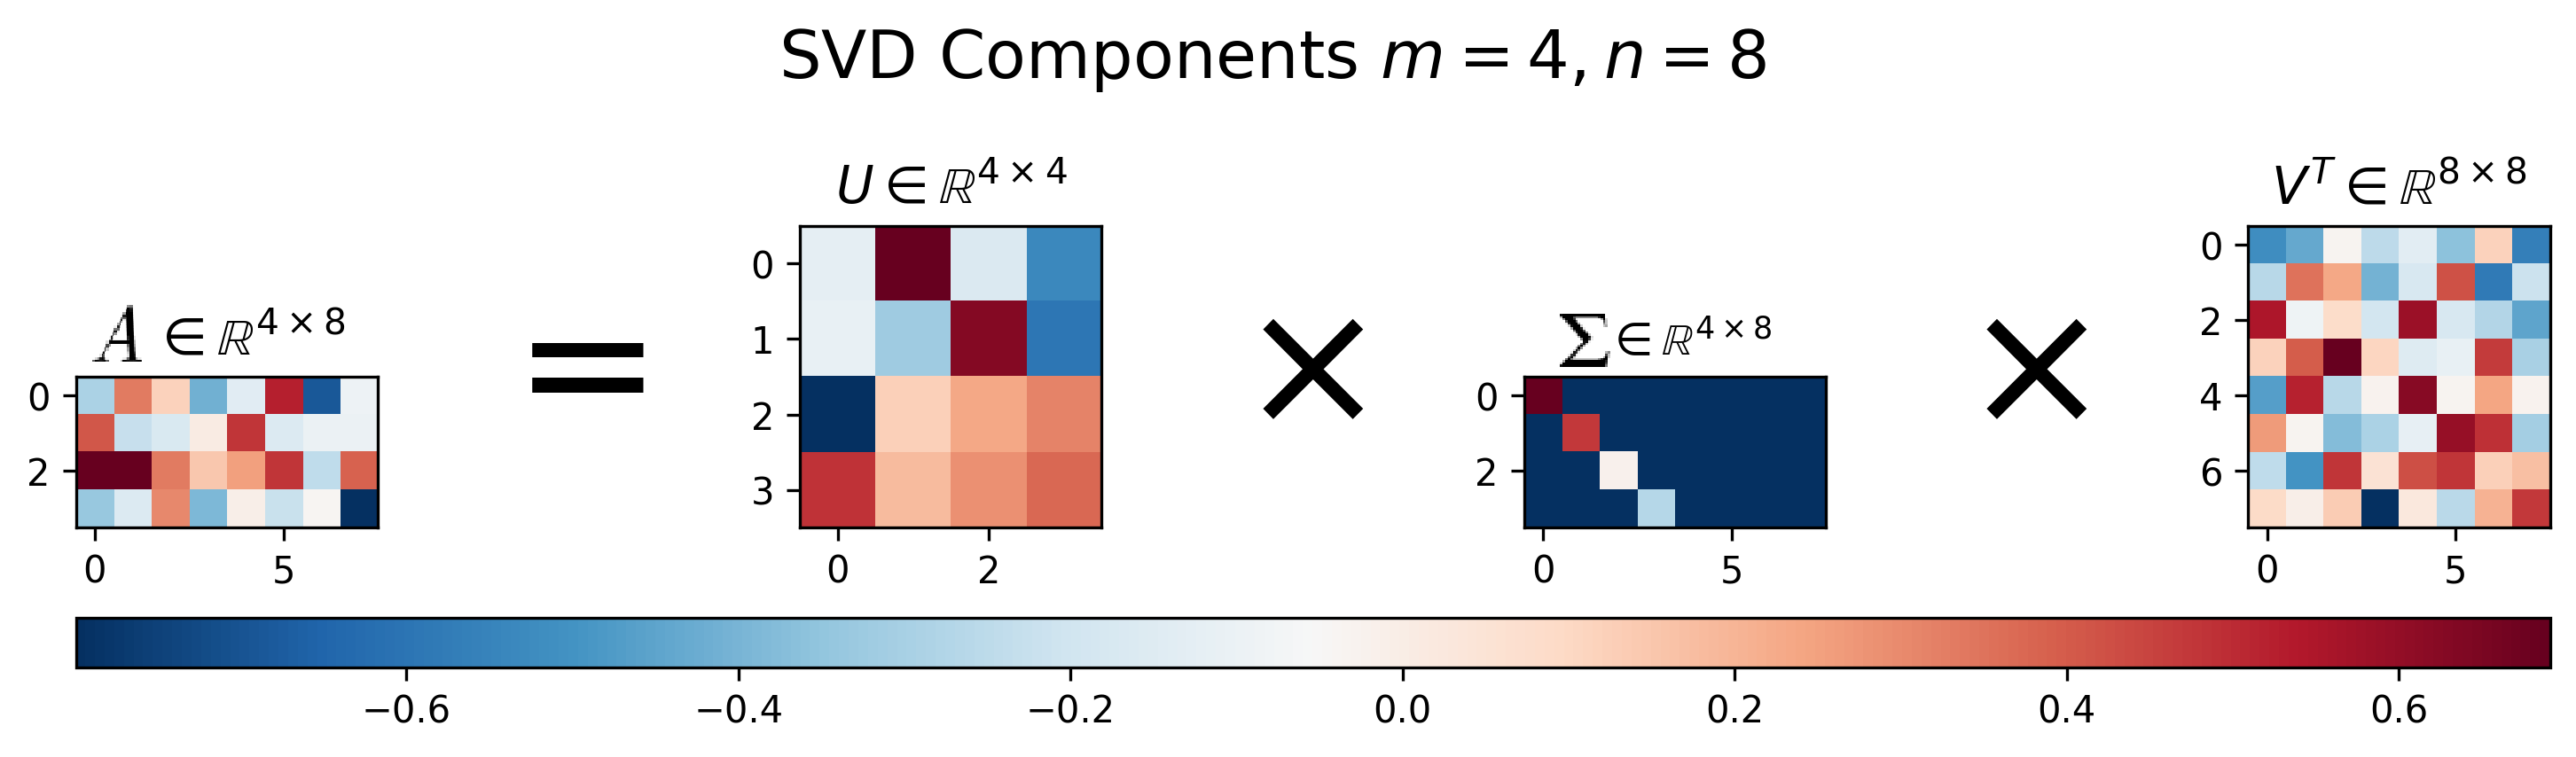
\includegraphics[scale=0.3]{svdm_nho_n}
	\caption{\textit{Biểu diễn SVD của ma trận A khi m<n}}\label{fig:Picture}
\end{figure}\\

\textbf{\textcolor{blue}{Mô tả SVD của ma trận A trong trường hợp m>n (m=8 và n=4)}} \\
\begin{figure}[!ht]
	\centering
	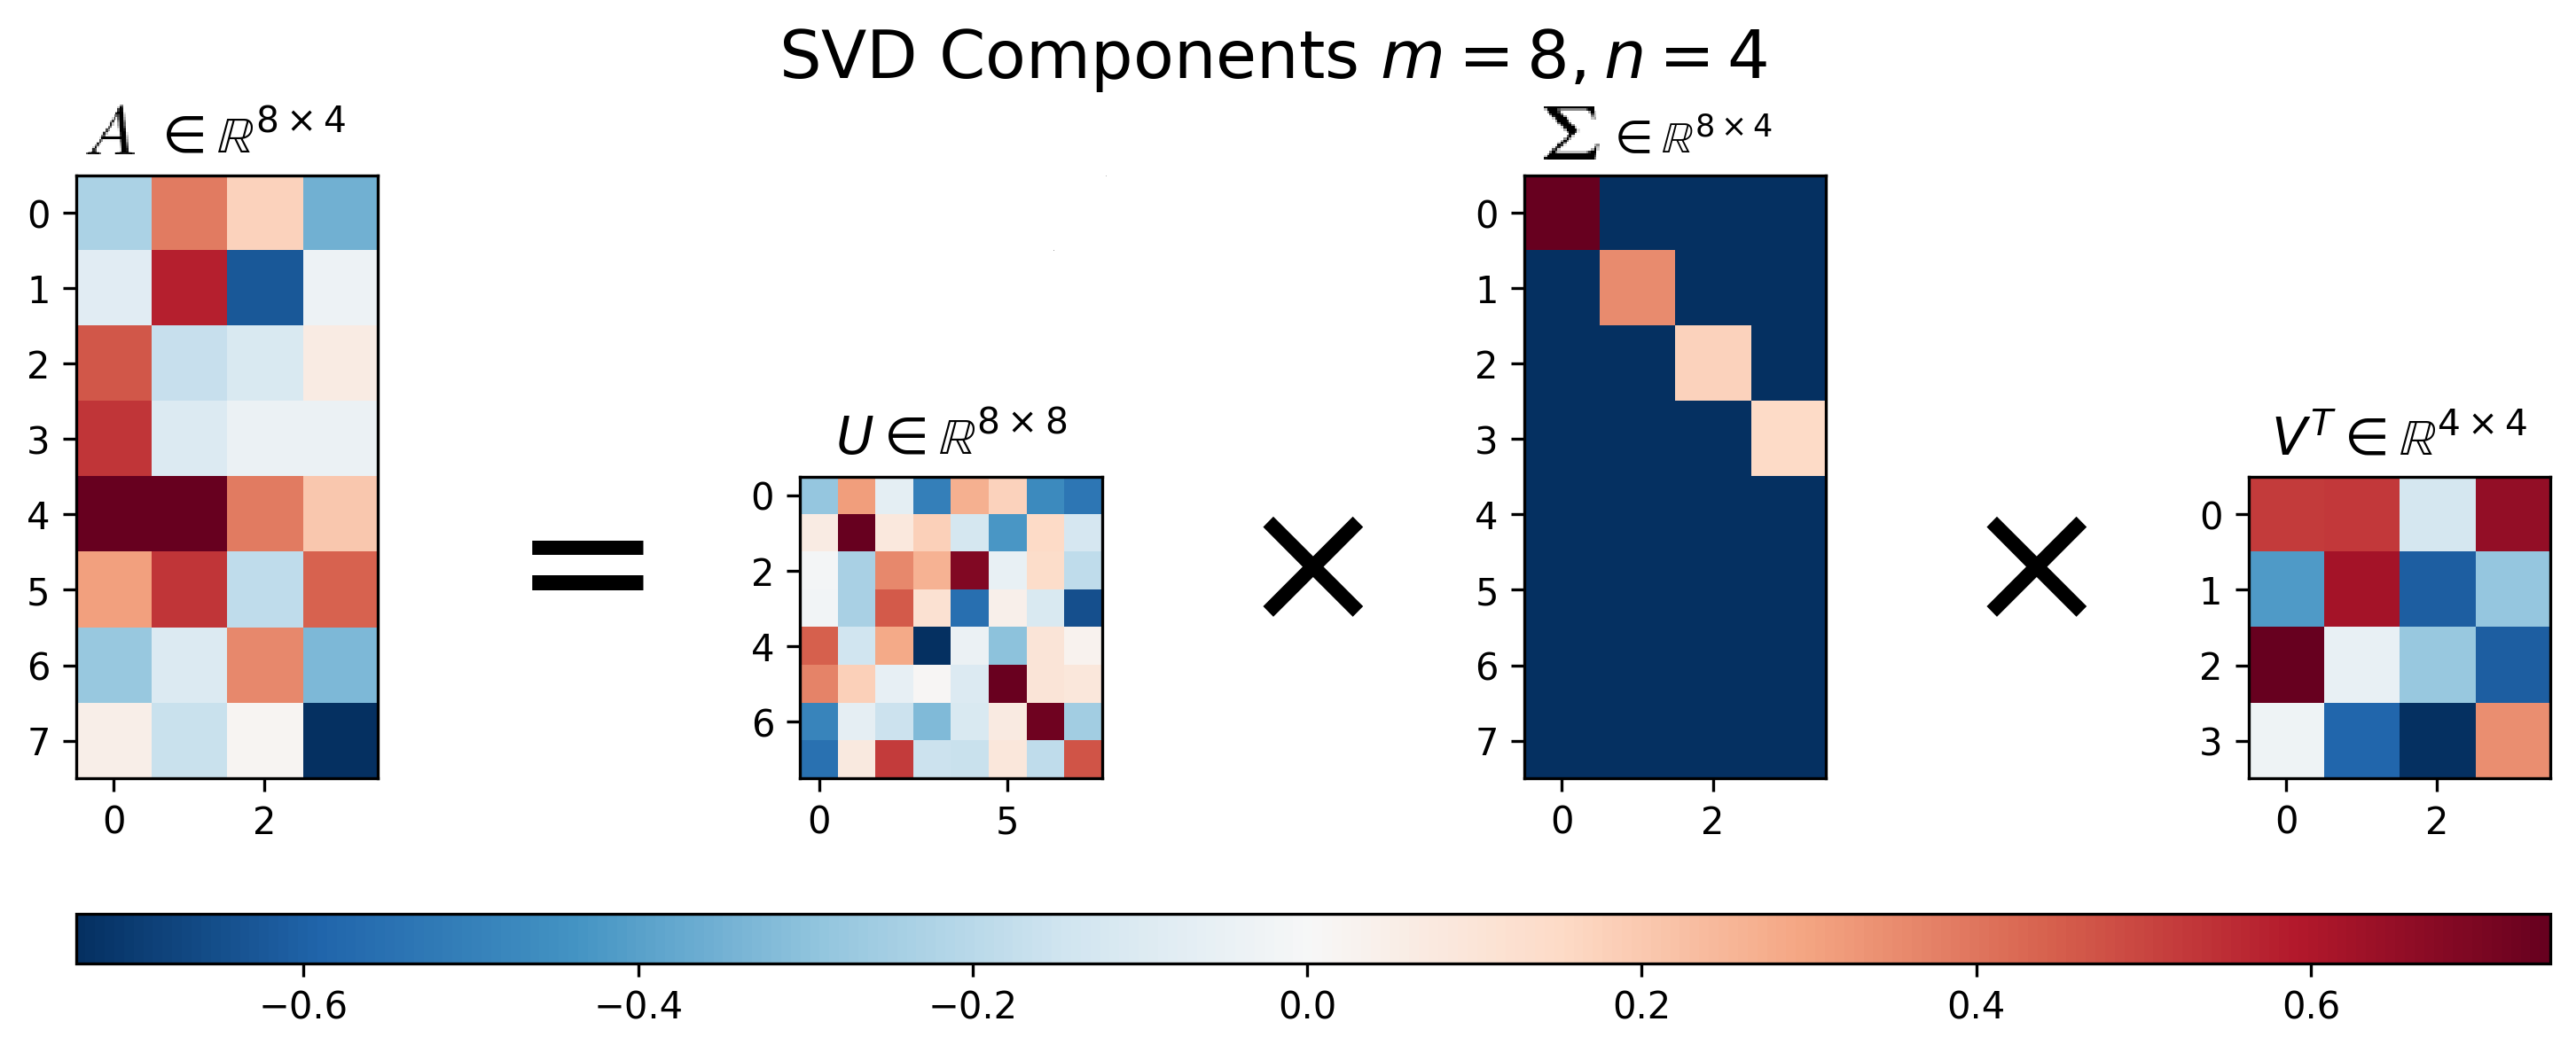
\includegraphics[scale=0.3]{svdm_lon_n}
	\caption{\textit{Biểu diễn SVD của ma trận A khi m>n}}\label{fig:Picture}
\end{figure}
\\
\textbf{\textcolor{blue}{Mô tả SVD của ma trận A trong trường hợp m=n (m=n=4)}} \\
\begin{figure}[!ht]
	\centering
	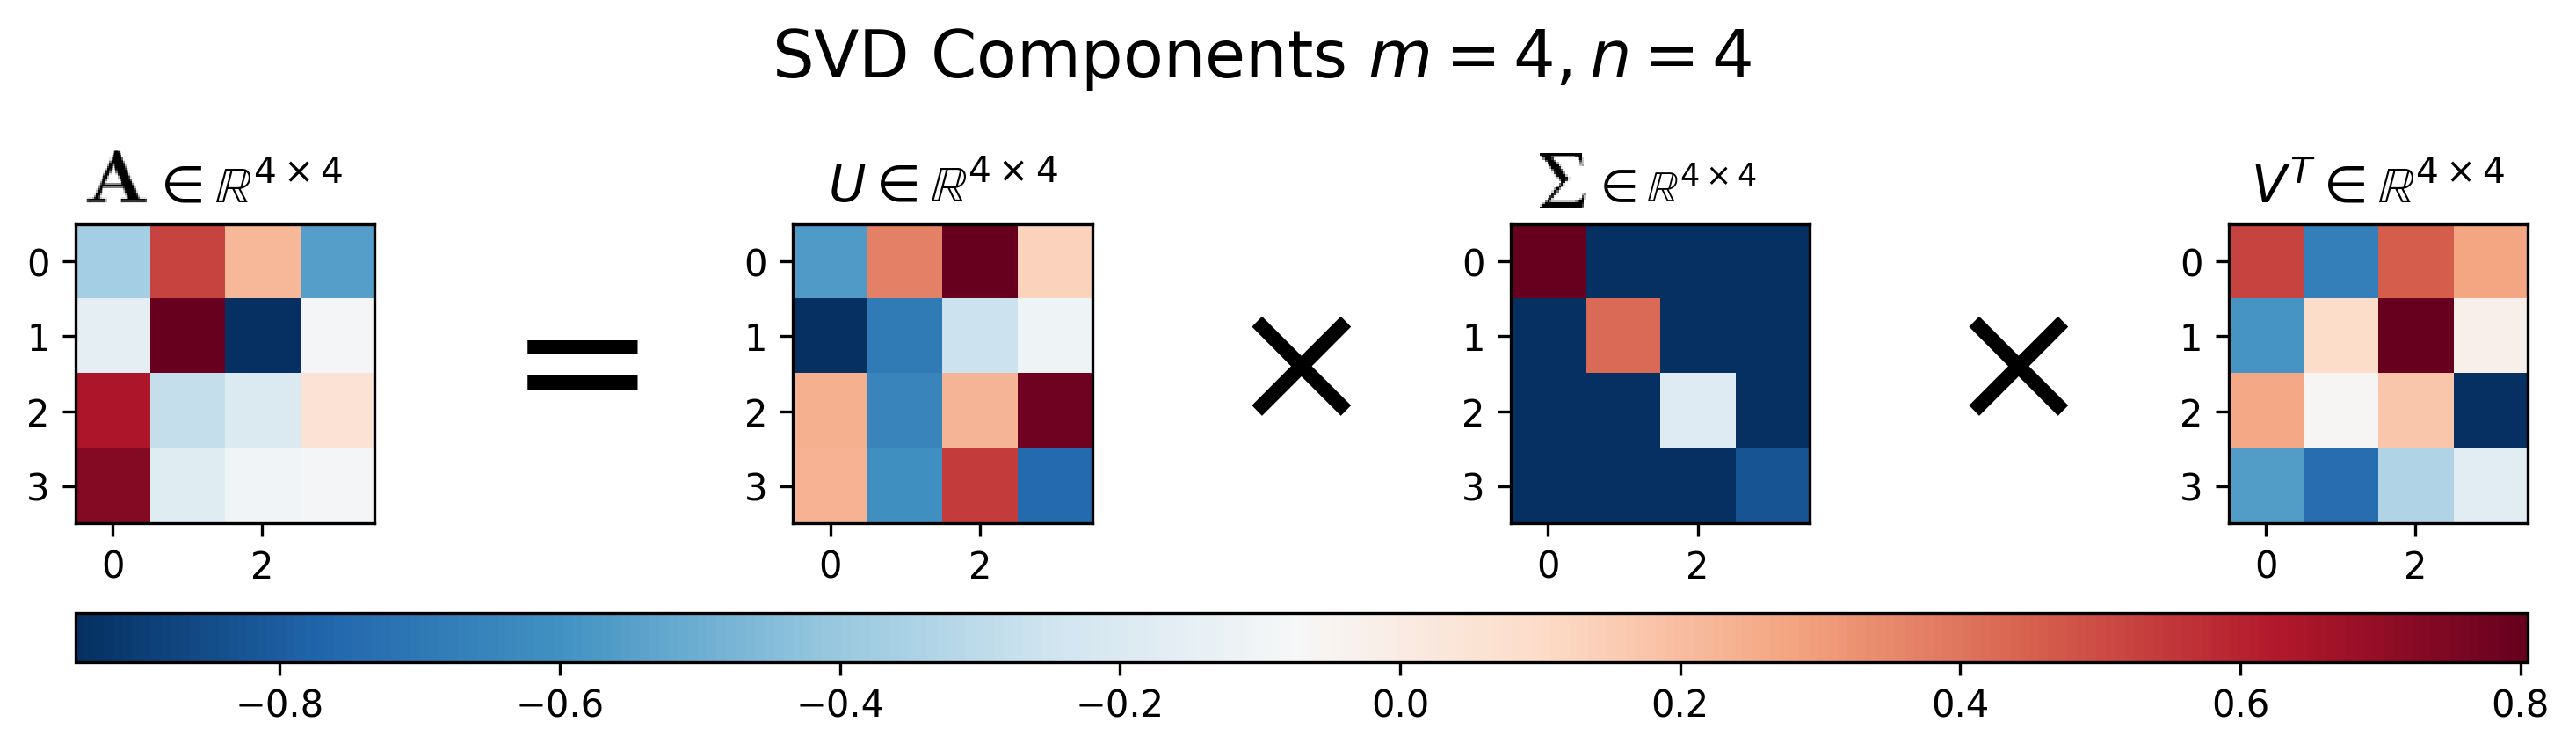
\includegraphics[scale=0.3]{svdm_bang_n}
	\caption{\textit{Biểu diễn SVD của ma trận A khi m=n}}\label{fig:Picture}
\end{figure}\\
\subsubsection{Nguồn gốc của SVD}
Từ công thức (5) ta có:\\
\begin{center}
	
	$
	\mathbf{AA}^T &=& \mathbf{U}\mathbf{\Sigma} \mathbf{V}^T (\mathbf{U}\mathbf{\Sigma} \mathbf{V}^T)^T &=& \mathbf{U}\mathbf{\Sigma} \mathbf{V}^T \mathbf{V}\mathbf{\Sigma}^T\mathbf{U}^T
	&=& \mathbf{U}\mathbf{\Sigma}\mathbf{\Sigma}^T\mathbf{U}^T =  \mathbf{U}\mathbf{\Sigma}\mathbf{\Sigma}^T\mathbf{U}^{-1} ~~~~~ (6)
	$
\end{center}\\
Dấu bằng cuối cùng xảy ra vì $\mathbf{V}^T\mathbf{V} = \mathbf{I}$ do $\mathbf{V}$  là một ma trận trực giao.\\
Quan sát thấy rằng $\Sigma\Sigma^T$  là một ma trận đường chéo với các phần tử trên đường chéo là $\sigma_1^2, \sigma_2^2, \dots$. Vậy (6)  chính là Eigen Decomposition của $\mathbf{A}\mathbf{A}^T$. Thêm nữa, $\sigma_1^2, \sigma_2^2, \dots$ chính là các trị riêng của $\mathbf{A}\mathbf{A}^T$.\\
Ma trận $\mathbf{A}\mathbf{A}^T$  luôn là ma trận nửa xác định dương nên các trị riêng của nó là không âm. Các $\sigma_i$  là căn bậc hai của các trị riêng của $\mathbf{A}\mathbf{A}^T$  còn được gọi là \textit{singular values}  của $\mathbf{A}$. Cái tên Singular Value Decomposition xuất phát từ đây.\\
Cũng theo đó, mỗi cột của $\mathbf{U}$ chính là một vector riêng của $\mathbf{A}\mathbf{A}^T$. Ta gọi mỗi cột này là \textit{left-singular vectors} của $\mathbf{A}$. Tương tự như thế, $\mathbf{A}^T\mathbf{A} = \mathbf{V}\Sigma^T\Sigma \mathbf{V}^T$ và các cột của $\mathbf{V}$  còn được gọi là các \textit{right-singular vectors} của $\mathbf{A}$\\  



\subsection{Các phép giảm chiều SVD}
Thông thường việc phân tích suy biến một ma trận có kích thước lớn sẽ rất lâu vì đòi hỏi phải giải phương trình đặc trưng để tìm ra các giá trị đặc trưng, từ đó suy ra ma trận đường chéo $\mathbf{\Sigma}$. Từ phương trình phân tích riêng $\mathbf{A^{T}A} = \mathbf{V\Sigma^{T}\Sigma V^T}$ suy ra $\mathbf{A^{T}AV} = \mathbf{V\Sigma^{T}\Sigma}$ , sử dụng phương trình ứng với từng cột cả 2 vế trái và phải để tính ra được các vector riêng ứng với mỗi trị riêng và suy ra được ma trận $\mathbb{V}$. Cách tìm ma trận $\mathbb{U}$ cũng được suy ra tương tự từ phương trình phân tích riêng  $\mathbf{A^{T}} = \mathbf{U\Sigma \Sigma^{T}U^T}$ . Quá trình này phải trải qua nhiều bước và khi kích thước ma trận lớn, chi phí thời gian và lưu trữ sẽ rất lớn. Vì vậy các dạng giảm chiều SVD sẽ rút gọn quá trình tính toán.

\subsubsection{Compact SVD}
Viết lại biểu thức (5) dưới dạng tổng của các ma trận rank 1: \\
\begin{center}
	$A=\sigma_1u_1v_1^T+\sigma_2u_2v_2^2+...+\sigma_ru_rv_r^T$
\end{center}
với chú ý rằng mỗi $u_iv_i^T, 1 \leq i \leq r $ là một ma trận có rank bằng 1\\
Rõ ràng trong cách biểu diễn này, ma trận $\mathbf{A}$ chỉ phụ thuộc vào r cột đầu tiên của $\mathbf{U, V}$ và r giá trị khác 0 trên đường chéo của ma trận $\Sigma$. Vì vậy ta có một cách phân tích \textit{gọn} hơn và gọi là \textit{compact SVD}:\\
\begin{center}
	$
	\mathbf{A} = {\mathbf{U}}_r{\Sigma}_r({\mathbf{V}}_r)^T$
\end{center} 
Với $\mathbf{U}_r, \mathbf{V}_r $ lần lượt là ma trận được tạo bởi r cột đầu tiên của $\mathbf{U}$ và $\mathbf{V}$. $\Sigma_r$ là ma trận con được tạo bởi r hàng đầu tiên và r cột đầu tiên của $\Sigma$. Nếu ma trận $\mathbf{A}$ có rank nhỏ hơn rất nhiều so với số hàng và số cột $r \ll m, n$, ta sẽ được lợi nhiều về việc lưu trữ.\\
Dưới đây là ví dụ minh hoạ với $m = 4, n = 6, r = 2$\\

\begin{figure}[!ht]
	\centering
	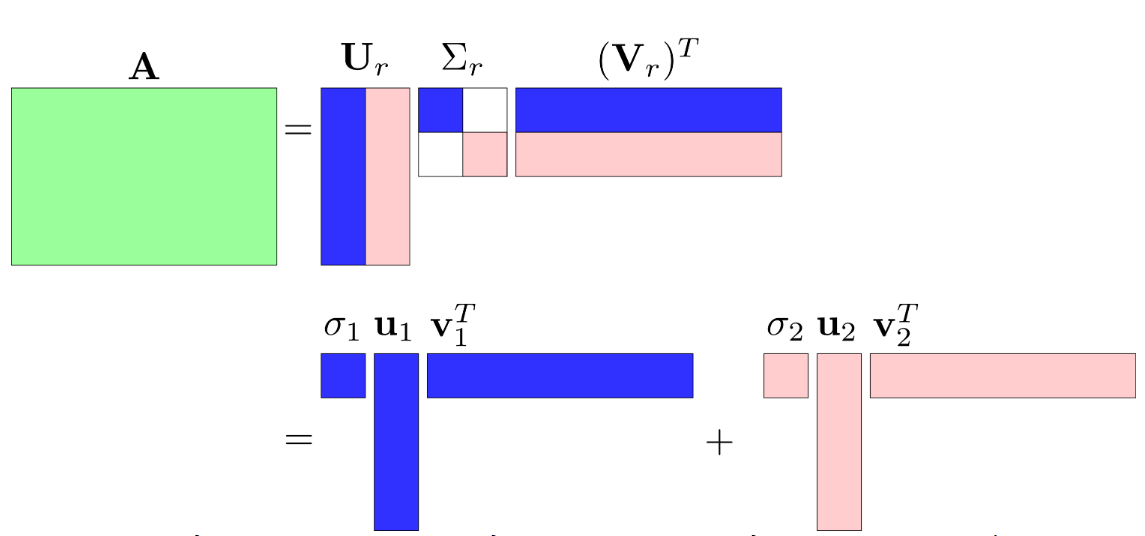
\includegraphics[scale=0.3]{svd_}
	\caption{\textit{Biểu diễn SVD dạng thu gọn và biểu diễn ma trận dạng tổng các ma trận có rank bằng 1.}}\label{fig:Picture}
\end{figure}\\

\subsubsection{Truncated SVD}
Chú ý rằng trong ma trận $\Sigma$, các giá trị trên đường chéo là không âm và giảm dần $\sigma_1 \geq \sigma_2 \geq \dots, \geq \sigma_r \geq 0 = 0 = \dots = 0$. Thông thường, chỉ một lượng nhỏ các $\sigma_i$ mang giá trị lớn, các giá trị còn lại thường nhỏ và gần 0. Khi đó ta có thể xấp xỉ ma trận $\mathbf{A}$ bằng tổng của $k < r$ ma trận có rank 1:\\
\begin{center}
	$
	\mathbf{A} \approx \mathbf{A}_k = \mathbf{U}_k \Sigma_k (\mathbf{V}_k)^T = \sigma_1 \mathbf{u}_1 \mathbf{v}^T_1 + \sigma_2\mathbf{u}_2\mathbf{v}_2^2 + \dots + \sigma_k\mathbf{u}_k\mathbf{v}k^T ~~~~ (7)$
\end{center}

Định lý dưới đây nói rằng sai số do cách xấp xỉ trên chính là căn bậc hai của tổng bình phương của các singular values mà ta đã bỏ qua ở phần cuối của $\Sigma$. Ở đây sai số được định nghĩa là Frobineous norm của hiệu hai ma trận:\\
\textbf{Định lí}\\
\begin{center}
	$
	||\mathbf{A} - \mathbf{A}_k||_F^2 = \sum_{i = k + 1}^r \sigma_i^2 ~~~ (8)$
\end{center}
\\\textit{Chứng minh}\\
Sử dụng tính chất $||\mathbf{X}||_F^2 = \text{trace}(\mathbf{X}\mathbf{X}^T)$ và $\text{trace}(\mathbf{XY}) = \text{trace}(\mathbf{YX})$ với mọi ma trận $\mathbf{X, Y}$ ta có:\\

$
||\mathbf{A} - \mathbf{A}_k||_F^2 & = & ||\sum_{i = k + 1}^r \sigma_i \mathbf{u}_i\mathbf{v}_i^T ||_F^2    & (9)\
& = & \text{trace}\left\{ \left(\sum_{i = k + 1}^r \sigma_i \mathbf{u}_i\mathbf{v}_i^T\right)
\left(\sum_{j = k + 1}^r \sigma_j \mathbf{u}_j\mathbf{v}_j^T\right)^T
\right\} & (10) \\
&=& \text{trace}\left\{ \sum_{i = k + 1}^r \sum_{j = k + 1}^r \sigma_i\sigma_j \mathbf{u}_i\mathbf{v}_i^T \mathbf{v}_j \mathbf{u}_j^T
\right\} & (11) \ 
&=& \text{trace}\left\{ \sum_{i = k + 1}^r  \sigma_i^2\mathbf{u}_i\mathbf{u}_i^T
\right\} & (12) \\
&=& \text{trace}\left\{ \sum_{i = k + 1}^r  \sigma_i^2\mathbf{u}_i^T\mathbf{u}_i
\right\} & (13) \ 
&=& \text{trace}\left\{ \sum_{i = k + 1}^r  \sigma_i^2
\right\} & (14) \ 
& = & \sum_{i = k + 1}^r \sigma_i^2 & (15)
$\\
\\
Dấu bằng ở (12) là vì $\mathbf{V}$ là ma trận trực giao (xem (4))\\
Dấu bằng ở (13) là vì hàm \text{trace} có tính chất giao hoán.\\
Dấu bằng ở (15) là vì biểu thức trong dấu ngoặc của (14)  là một số vô hướng.\\

\\Thay $k=0$ ta sẽ có:\\
\begin{center}
	$||\mathbf{A}||_F^2 = \sum_{i = 1}^r \sigma_i^2~~~~ (16) $
\end{center} 
Từ đó:\\
\begin{center}
	$
	\dfrac{||\mathbf{A} - \mathbf{A}_k||_F^2}{||\mathbf{A}||_F^2} = {\dfrac{\sum_{i = k + 1}^r \sigma_i^2}{\sum_{j = 1}^r \sigma_j^2}} ~~~~ (17)$
\end{center}
\\
Như vậy, \textbf{ Đây là một định lý quan trọng giúp xác định việc xấp xỉ ma trận dựa trên lượng thông tin muốn giữ lại.}\\
Ví dụ, nếu ta muốn giữ lại ít nhất 90\% lương thông tin trong $\mathbf{A}$, trước hết ta tính $\sum_{j = 1}^r \sigma_j^2$, sau đó chọn $k$ là số nhỏ nhất sao cho:\\
\begin{center}
	$
	\dfrac{\sum_{i = 1}^k \sigma_i^2}{\sum_{j = 1}^r \sigma_j^2} \geq 0.9$
\end{center}
\\
Khi $k$ nhỏ, ma trận $\mathbf{A}_k$ có rank là $k$, là một ma trận có rank nhỏ. Vì vậy, Truncated SVD còn được coi là một phương pháp \textit{Low-rank approximation}\\

\subsubsection{Best Rank k Approximation}
Người ta chứng minh được rằng (Singular Value Decomposition - Princeton) $\mathbf{A}_k$ chính là nghiệm của bài toán tối ưu:\\
\begin{center}
	$
	
	\min_{\mathbf{B}} &&||\mathbf{A} - \mathbf{B}||_F \ 
	\text{s.t.} && \text{rank}(\mathbf{B}) = k ~~~~~~~~~~~~~~ (17)
	$
\end{center}\\
và như đã chứng minh ở trên $||\mathbf{A} - \mathbf{A}_k||_F^2 = \sum_{i = k + 1}^r \sigma_i^2$\\
Nếu sử dụng norm 2 của ma trận thay vì Frobenius norm để đo sai số, $\mathbf{A}_k$ cũng là nghiệm của bài toán tối ưu:\\
\begin{center}
	
	$
	\min_{\mathbf{B}} &&||\mathbf{A} - \mathbf{B}||_2 \ 
	\text{s.t.} && \text{rank}(\mathbf{B}) = k ~~~~~~~~~~~~~~ (18)
	$
\end{center}\\
và sai số: $||\mathbf{A} - \mathbf{A}_k||_2^2 = \sigma_{k+1}^2$.
Định nghĩa của norm 2 của một ma trận là:\\
\begin{center}
	$
	||\mathbf{A}||_2 = \max_{||\mathbf{x}||_2 = 1} ||\mathbf{Ax}||_2
	$
\end{center}\\
Đây là lý do căn bậc hai của tổng bình phương của các phần tử của một ma trận không được gọi là norm 2 như đối với vector.\\
\begin{center}
	$
	||\mathbf{A}||_2 = \sigma_1$
\end{center}
\\
\textbf{Frobenius norm và norm 2 là hai norms được sử dụng nhiều nhất trong ma trận. Như vậy, xét trên cả hai norm này, Truncated SVD đều cho xấp xỉ tốt nhất. Vì vậy Truncated SVD còn được gọi là Best low-rank Approximation.}

\section{ỨNG DỤNG SVD VÀO KHỬ NHIỄU ÂM THANH}
\subsection{Đặt vấn đề}
Với cuộc sống của chúng ta hiện nay, thì rất quen thuộc chính là những âm thanh xung quanh với từng hoàn cảnh khác nhau như: tiếng của giảng viên trong buổi giảng bài trên lớp; âm thanh trong buổi hòa nhạc; tiếng nói phát ra trong cuộc trò chuyện,...
\\
\begin{figure}[!ht]
	\begin{minipage}[b]{0.4\textwidth}
		\centering
		
\includegraphics[scale=0.125]{amthanh}
		%\caption{\textit{Tốc độ tăng/giảm GDP}}\label{fig:*1}
	\end{minipage}
	\hfill
	\begin{minipage}[b]{0.4\textwidth}
		\centering
		
\includegraphics[scale=0.28]{amthanh2}
		%\caption{\textit{Cơ cấu GDP năm 2021}}\label{fig:*2}
	\end{minipage}
\end{figure}\\
Chúng ta thường ghi lại video hoặc những âm thanh cần thiết đến khi cần thì dùng lại, hiện nay thì điện thoại thông minh và các thiết bị ghi âm đã phát triển và có thể phục vụ nhu cầu đó của chúng ta. Tuy nhiên, có một điều khó có thể tránh khỏi đó là những tạp âm (tiếng gió, tiếng ồn, tiếng chó sủa,...) khiến cho chất lượng âm thanh giảm gây khó chịu cho người nghe hoặc tạp âm quá nhiều khiến chúng ta không thể nghe được nội dung chính cần nghe lại\\
Vậy vấn đề đặt ra là làm thế nào để loại bỏ những tạp âm đó hay còn gọi là khử nhiễu giúp nâng cao chất lượng âm thanh tốt hơn có thể\\

\subsection{Khử nhiễu âm thanh dùng SVD}
\begin{itemize}
	\item Hiện nay chúng ta có khá nhiều phần mềm và ứng dụng hỗ trợ việc xử lí âm thanh, đặc biệt là tính năng khử nhiễu. Có thể kể đến như AudioDroid, Ringtone Editor, WavePad Sound Editor,... Các phần mềm này thường được viết dựa trên mã nguồn xử lí nhiễu âm thanh của các ngôn ngữ lập trình như C/C++, Python, Matlab,...Trên phương diện báo cáo, nhóm tác giả sẽ thực hiện khử nhiễu âm thanh ứng dụng SVD của Matlab
	\item Về thuật toán: trong Matlab có rất nhiều phương pháp khác nhau, cũng như hỗ trợ các thuật toán để thực hiện khử nhiễu âm thanh như phân tích PCA, biến đổi Fourier hữu hạn, phân tích SVD,... Tuy nhiên việc khử nhiễu âm thanh bằng SVD có nhiều ưu điểm, thông qua việc biến đổi dữ liệu mới trong không gian mà vẫn đảm bảo được hạng của ma trận và kích thước các nhân tử của ma trận trong một giới hạn cho phép. Như vậy nhờ vào thuật toán này, chúng ta có thể xóa bỏ những vết nhiễu của âm thanh, từ đó giúp đầu ra của âm thanh chất lượng hơn
\end{itemize}
\subsection{Quá trình khử nhiễu âm thanh bằng SVD dùng Matlab}
\textbf{\textcolor{red}{Các bước phân tích SVD cho một file âm thanh trên Matlab}}\\
1. Đọc file âm thanh (định dạng wav, mp3,...) vào Matlab sử dụng lệnh \textbf(audioread)\\
\textbf{[Y,Hz] = audioread('input.wav');} \\
Với $Y$ là giá trị mẫu, $Hz$ là tần số của mẫu\\
\\
2. Chúng ta có thể nghe thử để kiểm tra file âm thanh vừa với đọc vào Matlab dùng lệnh (sound)\\
\textbf{sound(Y,Hz);}\\
\\
3. Vẽ biểu đồ cho file âm thanh để trực quan hơn, dễ quan sát hơn dùng lệnh (plot)\\
\textbf{t = 0:1/Hz:(length(Y)-1)/Hz;\\
figure('name','Do thi cua am thanh goc ban dau');\\
xlabel('Thoi gian (s)');\\
ylabel('Bien do tin hieu');\\
title('Do thi cua am thanh goc ban dau');\\
plot(t, Y);
}\\
\\

\begin{figure}[!ht]
	\begin{minipage}[b]{0.4\textwidth}
		\centering
		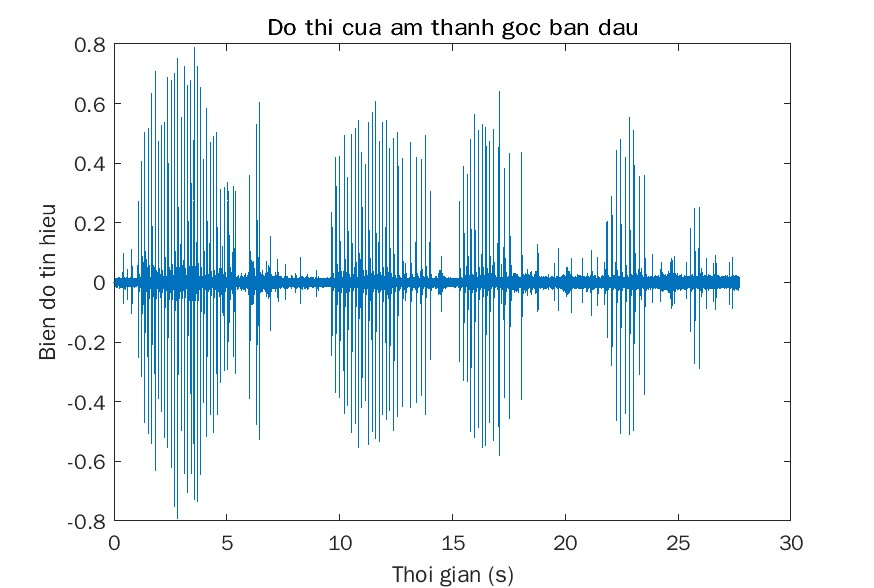
\includegraphics[scale=0.33]{goc1}
		%\caption{\textit{Tốc độ tăng/giảm GDP}}\label{fig:*1}
	\end{minipage}
	\hfill
	\begin{minipage}[b]{0.4\textwidth}
		\centering
		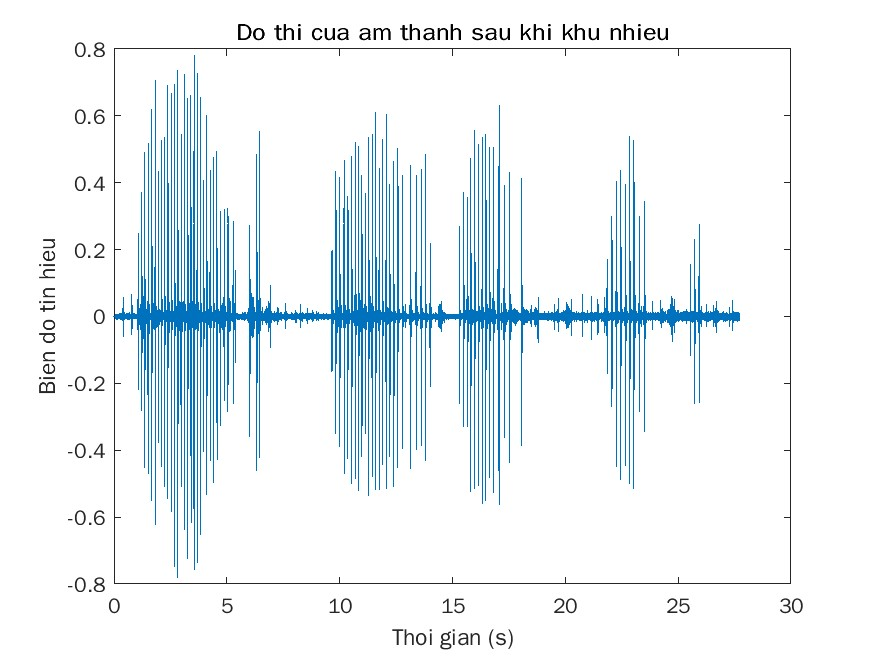
\includegraphics[scale=0.3]{khu}
		%\caption{\textit{Cơ cấu GDP năm 2021}}\label{fig:*2}
	\end{minipage}
\end{figure}\\
4. Tiến hành phân tích SVD để khử đoạn âm thanh bị nhiễu đó. Mã hóa thành một ma trận gồm các nhân tử để nhận dạng được, từ dó phân tích SVD để khử nhiễu\\
Chuyển âm thanh về dạng ma trận X với tỉ lệ nhỏ hơn để phân tích, vì kích thước của Y rất lớn (888582, 1) nên không thể tính toán trên ma trận này, ta dùng lệnh (reshape):\\
\textbf{
	X = reshape(Y,[\hspace{0.2cm}],822);\\
}
\\
Phân tích SVD của ma trận X với lệnh (svd) do Matlab cung cấp sẵn\\
\textbf{
	[U,S,V] = svd(X);
}.\\
Với U, V là các ma trận trực giao, S là ma trận đường chéo như đã phân tích trong phần cơ sở lí thuyết trước đó\\
\newpage 
5. Qua quá trình phân tích ma trận A thành SVD, chọn các điểm trong không gian chính là những đoạn bị tạp âm để xử lí. Sau khi xử lí hoàn tất, ta dùng câu lệnh “figure, subplot” để hiển thị đoạn âm thanh mà ta vừa xử lí, để đối chiếu so sánh. \\

\begin{figure}[!ht]
	\begin{minipage}[b]{0.4\textwidth}
		\centering
		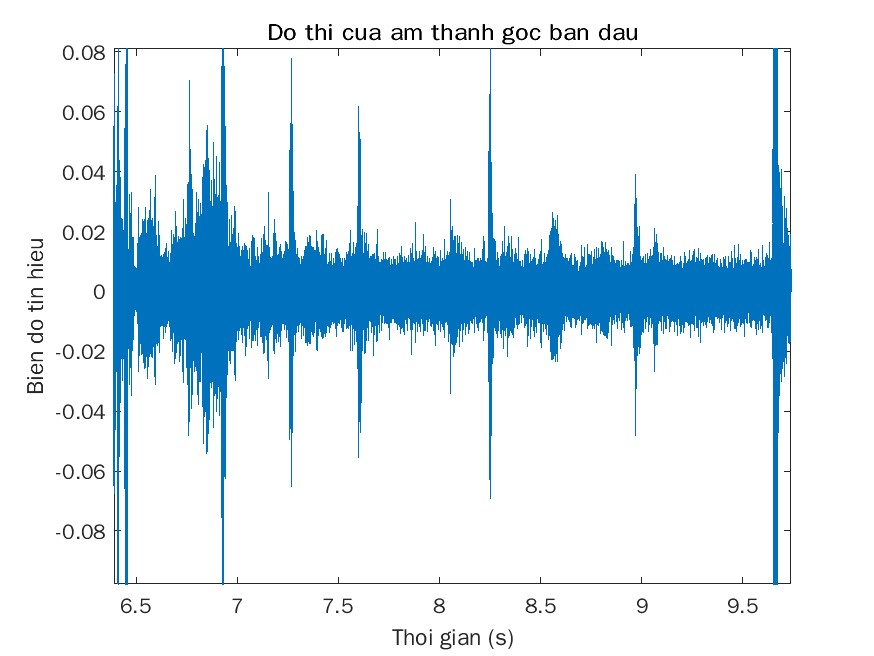
\includegraphics[scale=0.3]{goc_zoom}
		%\caption{\textit{Tốc độ tăng/giảm GDP}}\label{fig:*1}
	\end{minipage}
	\hfill
	\begin{minipage}[b]{0.4\textwidth}
		\centering
		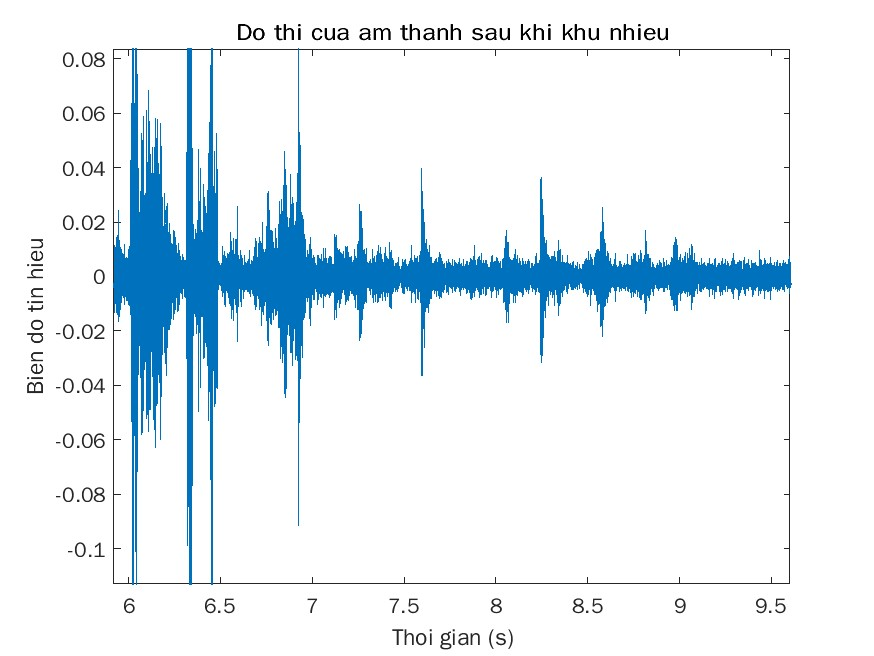
\includegraphics[scale=0.3]{khu_zoom}
		%\caption{\textit{Cơ cấu GDP năm 2021}}\label{fig:*2}
	\end{minipage}
\end{figure}\\

\subsection{Mã nguồn Matlab}
\begin{lstlisting}
	
	clear all; close all; clc;
	% Doc va tien xu l file am thanh
	[audio,Hz] = audioread('input.wav');
	X = reshape(audio,[],822);
	% Phan tich SVD
	[U,S,V] = svd(X);
	% Ve do thi am thanh goc ban dau
	t = 0:1/Hz:(length(audio)-1)/Hz;
	figure('name','Do thi cua am thanh goc ban dau');
	plot(t,audio);
	xlabel('Thoi gian (s)');
	ylabel('Bien do tin hieu');
	title('Do thi cua am thanh goc ban dau');
	% Chay va nghe doan am thanh goc
	sound(audio,Hz);
	pause(20);
	
	% Qua trinh khu nhieu
	reduction_diagonal_line = diag(S);
	reduction_diagonal_line(80:end) = 0;
	len_S = length(reduction_diagonal_line);
	reduction_S = S;
	reduction_S(1:len_S,1:len_S) = diag(reduction_diagonal_line);
	new_X = U*reduction_S*transpose(V);
	new_audio = reshape(new_X,[],2);
	new_audio = fillmissing(new_audio,'previous');
	new_audio_=reshape(new_audio, [888582,1])
	figure('name','Do thi cua am thanh sau khi khu nhieu');
	t = 0:1/Hz:(length(audio)-1)/Hz;
	plot(t,new_audio_);
	title('Do thi cua am thanh sau khi khu nhieu');
	xlabel('Thoi gian (s)');
	ylabel('Bien do tin hieu');
	sound(new_audio_,Hz);

\end{lstlisting}
\\
\textbf{\textcolor{red}{Một số lệnh đã sử dụng}}\\
- \textcolor{blue}{clear all}: Xóa các biến, dữ liệu trước đó\\
- \textcolor{blue}{close all}: Đóng tất cả các cửa sổ, đồ thị đang mở.\\
- \textcolor{blue}{clc}: Xóa màn hình Command Line\\
- \textcolor{blue}{audioread('file name')}: Mở 1 file âm thanh cần khử nhiễu có sẵn trong máy tính.\\
- \textcolor{blue}{reshape}: Thay đổi hình dạng của một mảng mà không thay đổi dữ liệu.\\
- \textcolor{blue}{[U,S,V] = svd (A)}:  Phân tích SVD ma trận A.\\
- \textcolor{blue}{Sigmas= diag(S)}: Gán các giá trị trên đường chéo chính của ma trận S.\\
- \textcolor{blue}{plot}: Vẽ đồ thị .\\
- \textcolor{blue}{for i=1:length(rank) approx\_sigmas = sigmas}: Loại bỏ các trị riêng thấp.\\
- \textcolor{blue}{approx\_S = S}: Gắn trị riêng đã xử lí vào ma trận S.\\
- \textcolor{blue}{xlabel, ylabel}:Đặt tên trục x, trục y.\\
- \textcolor{blue}{sound}: Lệnh phát âm thanh.\\
- \textcolor{blue}{Diag}: Lấy các giá trị trên đường chéo.\\
- \textcolor{blue}{Reduction\_diagonal\_line(80:end) = 0}: Khử các giá trị đường chéo từ hàng 80 trở đi về giá trị 0. \\
- \textcolor{blue}{Fillmissing}: Điền vào các giá trị trống vào các giá trị đứng trước đó.\\



\begin{figure}[!ht]
	\begin{minipage}[b]{0.4\textwidth}
		\centering
		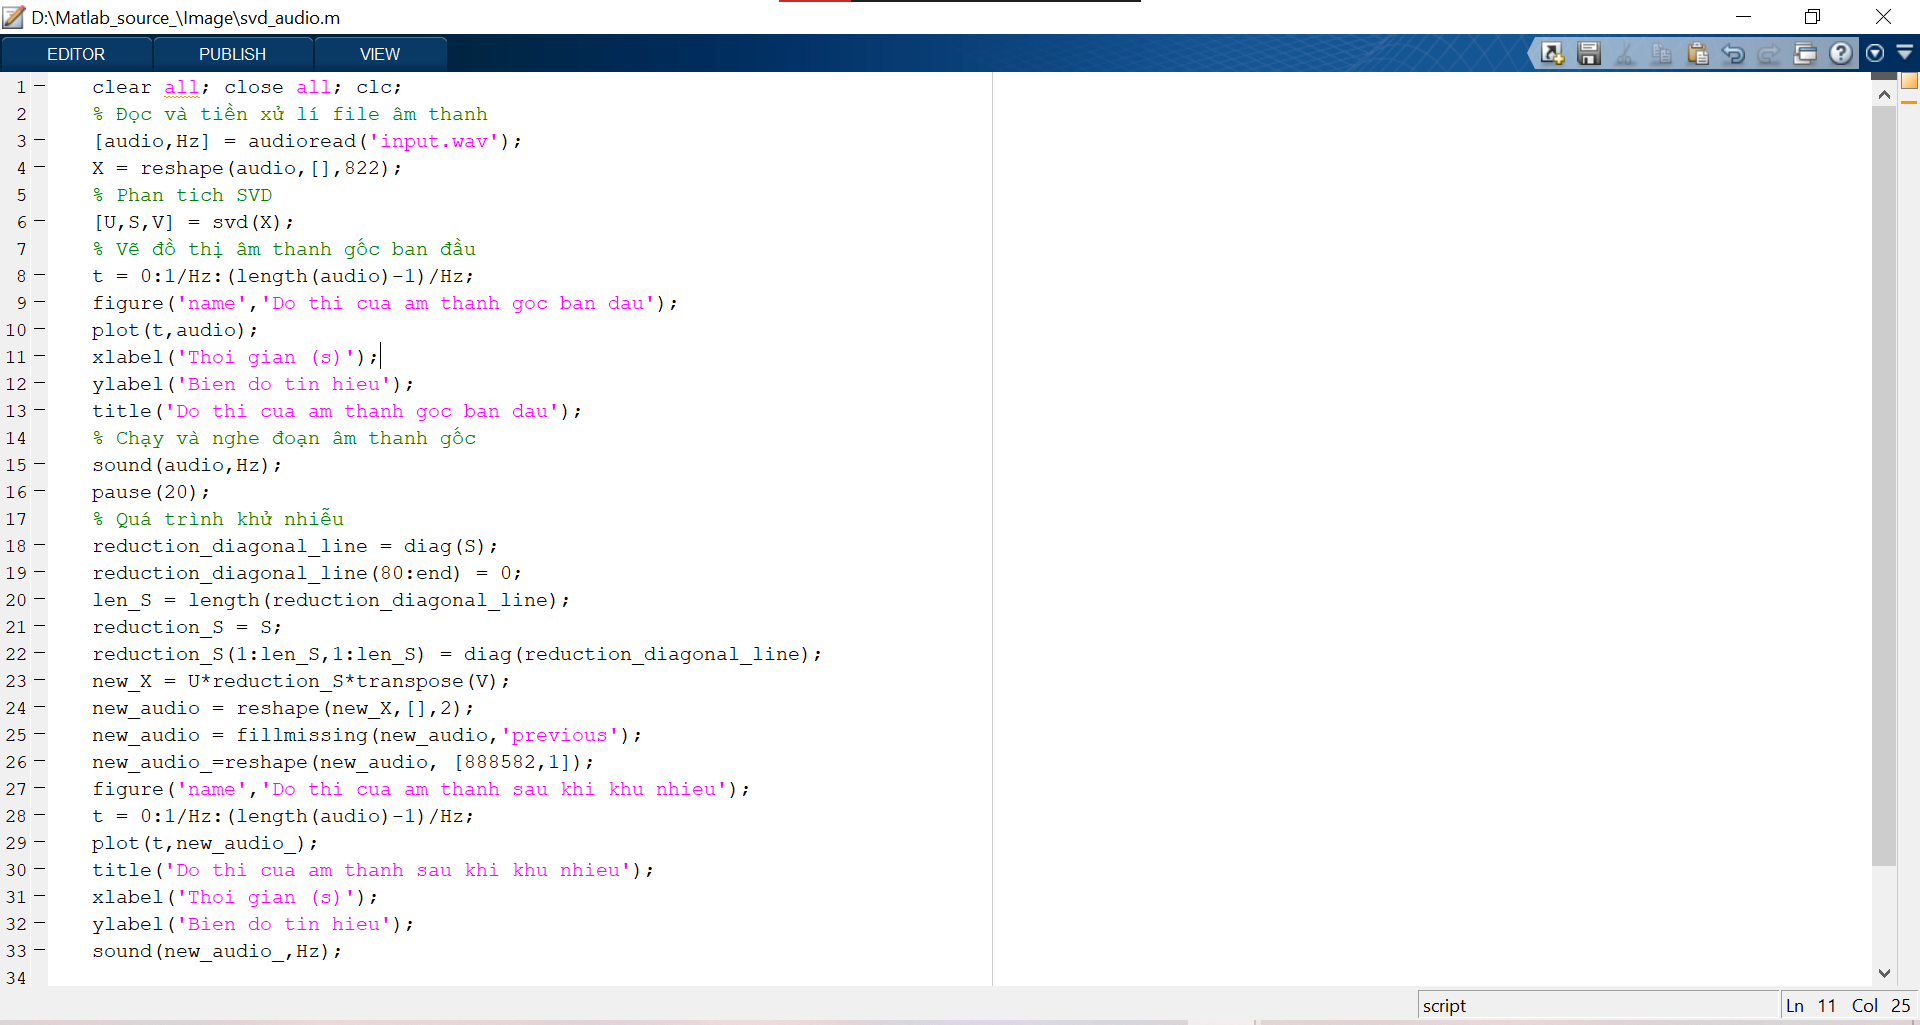
\includegraphics[scale=0.25]{code_}
		%\caption{\textit{Tốc độ tăng/giảm GDP}}\label{fig:*1}
	\end{minipage}
	
	\begin{minipage}[b]{0.4\textwidth}
		\centering
		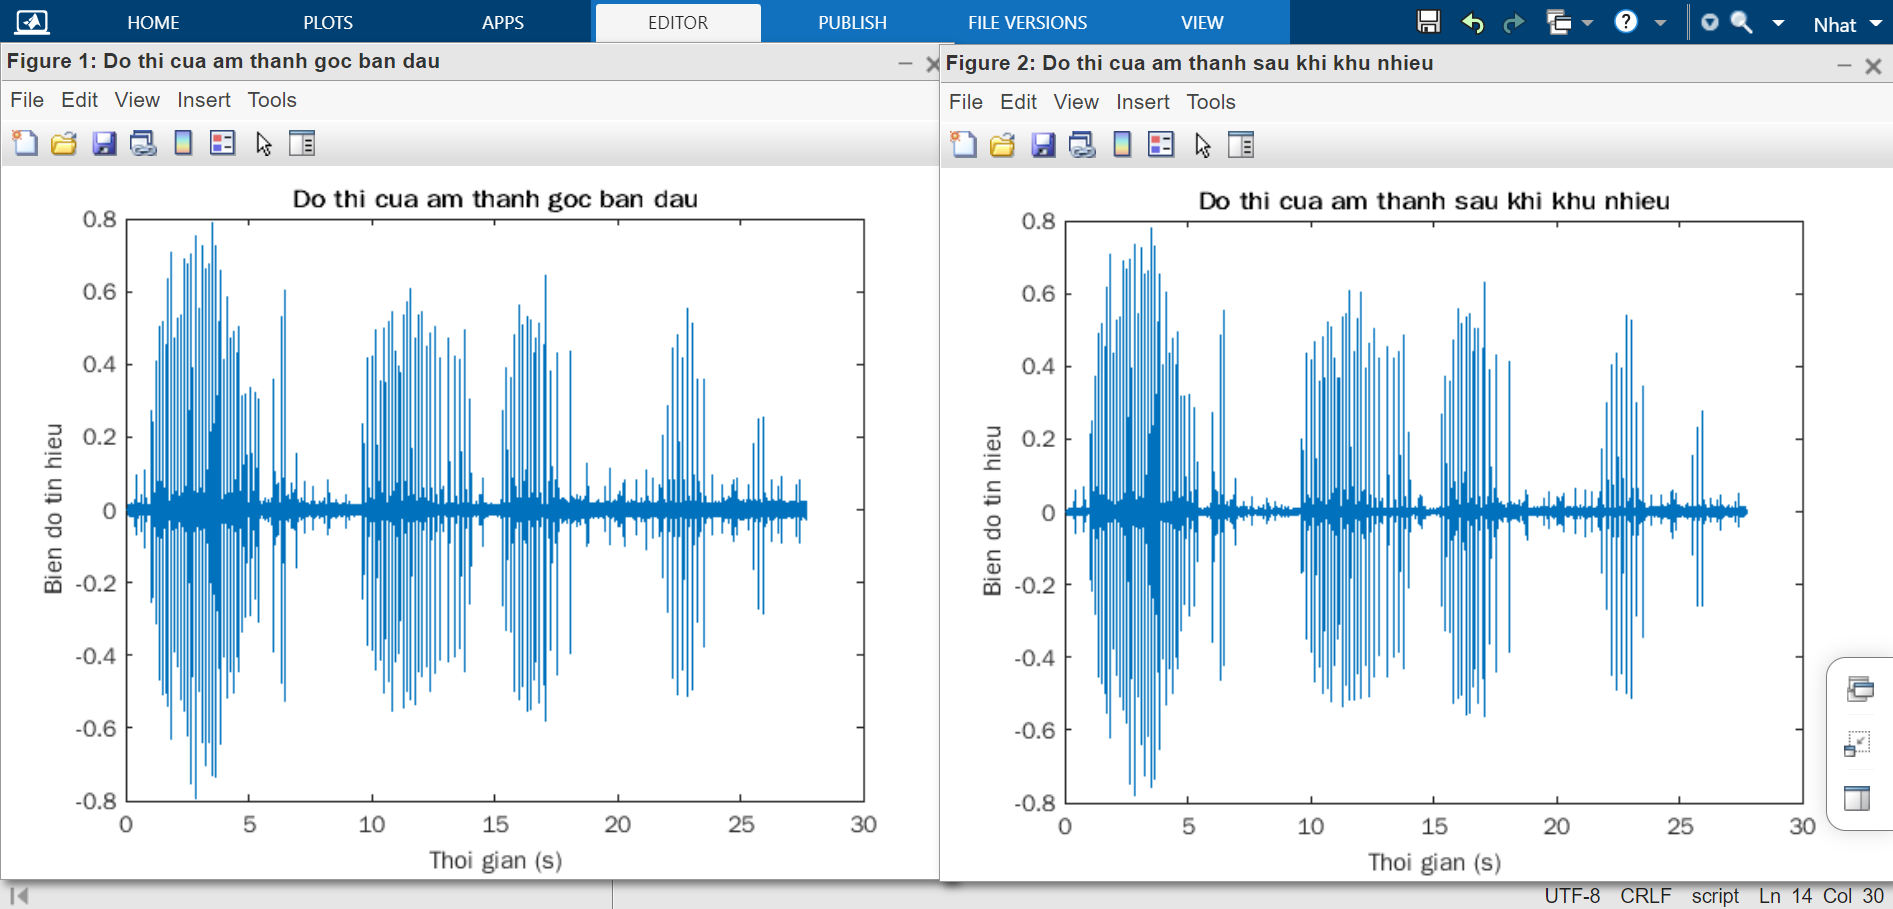
\includegraphics[scale=0.25]{code_kq}
		%\caption{\textit{Cơ cấu GDP năm 2021}}\label{fig:*2}
	\end{minipage}
\end{figure}\\










\section{MỘT VÀI ỨNG DỤNG KHÁC CỦA SVD}
\subsection{Image Compression (Nén hình ảnh)}

Giả sử ta có một tập dữ liệu nhiều ảnh có kích thước rất lớn. Khả năng lưu trữ của server là có hạn. Trong tình huống này ta có thể sau nén một bức ảnh bằng thuật toán truncate SVD để giảm kích thước của bộ ảnh vừa với dung lượng server mà thông tin của các bức ảnh vẫn giữ được một lượng lớn.\\
Để lưu ảnh với Truncated SVD, ta sẽ lưu các ma trận $\mathbf{U}_k \in \mathbb{R}^{m \times k}, \Sigma_k \in \mathbb{R}^{k \times k}, \mathbf{V}_k \in \mathbb{R}^{n \times k}$. Tổng số phần tử phải lưu là $k(m + n + 1)$ với chú ý rằng ta chỉ cần lưu các giá trị trên đường chéo của $4k(m + n + 1)$. Nếu so giá trị này với ảnh gốc có kích thước $mn$, mỗi giá trị là 1 số nguyên 1 byte, tỉ lệ nén là:\\
\begin{center}
	$
	\dfrac{4k(m + n + 1)}{mn}$
\end{center}\\
Khi $k \ll m, n$, ta có tỉ lệ nén xấp xỉ 0.69, tức đã tiết kiệm được khoảng 30\% bộ nhớ.\\

\begin{figure}[!ht]
	\centering
	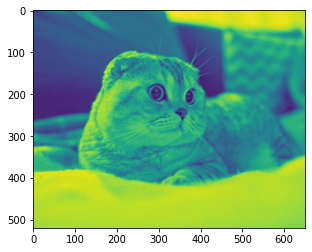
\includegraphics[scale=0.6]{goc}
	\caption{\textit{Bức ảnh gốc khi chưa nén}}\label{fig:Picture}
\end{figure}\\
Nén theo phương pháp SVD sao cho chỉ lấy lần lượt 10 trị riêng lớn nhất để lưu trữ thông tin \\
\begin{figure}[!ht]
	\centering
	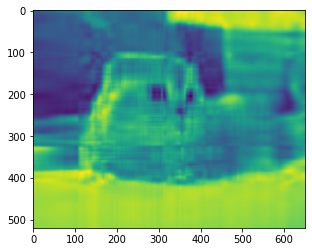
\includegraphics[scale=0.6]{10_}
	\caption{\textit{Nén ảnh với 10 trị riêng lớn nhất}}\label{fig:Picture}
\end{figure}\\

Nén theo phương pháp SVD sao cho chỉ lấy lần lượt 20 trị riêng lớn nhất để lưu trữ thông tin \\
\begin{figure}[!ht]
	\centering
	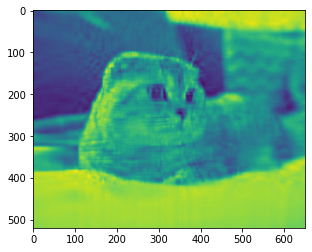
\includegraphics[scale=0.6]{20_}
	\caption{\textit{Nén ảnh với 10 trị riêng lớn nhất}}\label{fig:Picture}
\end{figure}\\

\subsection{Áp dụng cho thuật toán recommendation system}
Trong các thuật toán recommendation phương pháp SVD cũng tỏ ra hiệu quả hơn so với các phương pháp matrix factorization sử dụng gradient descent. Ý tưởng khi áp dụng vào recommendation system cũng tương tự như nén ảnh đó là căn cứ vào những cặp (user, item) đã được rating của ma trận tiện ích ta sẽ tìm ra một ma trận xấp xỉ tốt nhất với ma trận tiện ích. Sử dụng ma trận xấp xỉ để dự báo cho những cặp (user, item) chưa được rating.
\subsection{Giảm chiều dữ liệu }
Các ma trận $A_k$ gần khít với $A$ và có hạng bằng $k$ nên ta có thể dùng SVD để giảm chiều dữ liệu.\\
Việc giảm chiều dữ liệu giúp ta có khả năng biễu diễn bộ dữ liệu đó một cách khá chính xác trên đồ thị. Giả sử ta có một tập dữ liệu 4 chiều và ta muốn biểu diễn tập dữ liệu này trên đồ thị thì ta có thể dùng SVD để giảm chiều dữ liệu về 3.\\
Việc giảm chiều dữ liệu nhưng vẫn giữ được đặc trưng của bộ dữ liệu còn giúp số lượng tham số cần tính toán là ít hơn nên tính toán nhanh hơn.
\\
Ngoài các ứng dụng trên, SVD còn có các ứng dụng trong tối ưu cực trị rời rạc, lát cắt cực đại, K-means Clustering, Graph Partitioning, ... với một performance tính toán tương đối, rất thích hợp cho lượng dữ liệu lớn nhưng công dụng chính nhất vẫn là \textbf{giảm chiều dữ liệu}










































	\newpage 
	\addcontentsline{toc}{section}{Tài liệu tham khảo}
\begin{thebibliography}{99}
\bibitem{} CS168, {\it The Singular Value Decomposition (SVD)
		and Low-Rank Matrix Approximations}\\ \url{http://theory.stanford.edu/~tim/s15/l/l9.pdf}
\bibitem{} Kaggle, {\it Phương pháp phân tích suy biến.}\\ \url{https://www.kaggle.com/code/phamdinhkhanh/singular-value-decomposition/notebook}
\bibitem{} Machine learning cơ bản, {\it Bài 26: Singular Value Decomposition}\\ \url{https://machinelearningcoban.com/2017/06/07/svd/}
\bibitem{} Standford University, {\it Singular Value Decomposition}\\ \url{https://www.youtube.com/watch?v=P5mlg91as1c}


\bibitem{} Viblo, {\it [Handbook] Singular Values Decomposition và một số ứng dụng}\\ \url{https://viblo.asia/p/handbook-singular-values-decomposition-va-mot-so-ung-dung-yMnKMOoml7P}
\bibitem{} Mathwork, {\it QR decomposition: History and its
	Applications}\\ \url{https://www.mathworks.com/help/audio/ug/spectral-descriptors.html?searchHighlight=noise%20reduction%20audio%20code&s_tid=srchtitle}

\bibitem{} Youtube, {\it Lập trình Matlab xử lí âm thanh}\\ \url{https://www.youtube.com/watch?v=xXk9nS6YdU8&feature=youtu.be}
\bibitem{} Youtube, {\it MATLAB Tutorial for Beginners 43 - Audio Analysis Using MATLAB | Audio Analysis in MATLAB}\\ \url{https://www.youtube.com/watch?v=SJRHv5vvlnU}

\bibitem{} Vimach.net, {\it MATLAB cơ bản 9: Vecto (mảng) với file âm thanh}\\ \url{https://vimach.net/threads/matlab-co-ban-9-vecto-mang-voi-file-am-thanh.160/}

\end{thebibliography}
 
	
\end{document}



















